\documentclass[a4paper]{article}

\usepackage{graphicx}
\usepackage{float}
\usepackage{listings}
\usepackage{xcolor}
\usepackage{graphicx}

\definecolor{codegreen}{rgb}{0,0.6,0}
\definecolor{codegray}{rgb}{0.5,0.5,0.5}
\definecolor{codepurple}{rgb}{0.58,0,0.82}
\definecolor{backcolour}{rgb}{0.95,0.95,0.92}

\lstdefinestyle{mystyle}{
    backgroundcolor=\color{backcolour},   
    commentstyle=\color{codegreen},
    keywordstyle=\color{magenta},
    numberstyle=\tiny\color{codegray},
    stringstyle=\color{codepurple},
    basicstyle=\ttfamily\footnotesize,
    breakatwhitespace=false,         
    breaklines=true,    captionpos=b,                    
    keepspaces=true, numbers=left,                    
    numbersep=5pt, showspaces=false,                
    showstringspaces=false, showtabs=false, tabsize=2}
\lstset{style=mystyle}


\usepackage[utf8x]{inputenc}
\usepackage{fancyhdr}
\usepackage{lastpage}
% For figures and stuff
\usepackage{graphicx, wrapfig, subcaption, setspace, booktabs}
\usepackage[T1]{fontenc}
% Change for different font sizes and families
\usepackage[font=small, labelfont=bf]{caption}
\usepackage{fourier}
\usepackage[]{microtype}



\newcommand{\HRule}[1]{\rule{\linewidth}{#1}}
\onehalfspacing
\setcounter{tocdepth}{5}
\setcounter{secnumdepth}{5}

\usepackage[a4paper,top=2.5cm,bottom=2cm,left=2.5cm,right=2.5cm,marginparwidth=1.8cm]{geometry}
\pagestyle{fancy}


\setlength\headheight{15pt}
\fancyhead[L]{} 
\fancyhead[R]{Group 13}

\linespread{1.4}

%-----------------------------------------BEGIN DOC----------------------------------------
\begin{document}

\title{{\Huge \textbf{Technical Report}{\large\linebreak\\}}{\Large \textit{Effect of oven temperature and cooking time on \\resultant internal temperature of chicken breasts}\linebreak\linebreak}}

\author{Wenshan Cheng, Natalia Demidova, Zhirui Chu, \\ Lucas Noritomi-Hartwig, Hanshuo Ma, Matteo Giannone
\\ \\ \\
\textbf{University of Toronto at Missisauga} \\
Department of Mathematical \& Computational Sciences \\ \\
Professor Luai Al Labadi \\
STA305H5 S - Experimental Design \\ \\}
\date{\today}

\maketitle

\newpage
%-----------------------------------------CONTENT-------------------------------------
\tableofcontents\label{c}
\newpage
%-----------------------------------------ABSTRACT------------------------------------
% \begin{center}
% {\large\bf{Abstract\\}}
% \end{center}

% USDA food handling safety suggests the safe minimum internal temperature for all poultry products is 165 $^{\circ}$F or higher${^1}$. The purpose of this experiment lay in testing the significance of factors of oven temperature and oven cooking time in sufficiently predicting the internal temperature of cooked chicken breast. A completely randomized experiment design was employed, balanced by obtaining 10 observations of chicken internal temperature after each 4 treatments: combining cooking temperatures of 350${^\circ}$F, 375${^\circ}$F, and cooking times of 15, 20 minutes. It was found that ... The secondary purpose was investigating whether the final chicken breast temperature after cooking was influenced differently based on interaction of cooking time and temperature. It was found that ...

%--------------------------------------Introduction---------------------------------
\section{Introduction} \label{Introduction}
\vspace{-0.25cm}
\hspace{1cm}This study is concerned with one subtype of poultry product - chicken breasts, said to be safe to consume once the internal temperature reaches 165$^{\circ}$F\footnote{https://www.fsis.usda.gov/food-safety/safe-food-handling-and-preparation/food-safety-basics/safe-temperature-chart}. Chicken breasts are known to easily overcook and under-cook; overcooked breasts are dry and flavourless, and under-cooked breasts could lead to potential health issues through exposure to bacteria such as salmonella\footnote{https://www.cdc.gov/foodsafety/chicken.html}. This study aims to generate a basic cooking recipe for regular households to consume chicken breasts without taking the potential health risk, by investigating the effect of different combinations of oven temperature and cooking time on the resultant internal temperature of unseasoned, cut chicken breast. The desired outcome is a recipe that utilizes the least electrical energy (oven) and time, while successfully reaching safe internal temperature of chicken.

%-----------------------------------------Methodology------------------------------------
\section{Methodology} \label{Methodology}
\vspace{-0.25cm}

%-----------------------------------------Experimental Unit------------------------------------
\subsection{Experimental Unit}\label{Experimental Unit}
\vspace{-0.25cm}
\hspace{0.5cm}A piece of cut chicken breast.
%-----------------------------------------Description------------------------------------
\subsection{Description of Variables}\label{Description}
\vspace{-0.25cm}
\begin{itemize}
	\item{\textbf{(Y) Internal Temperature: }Internal temperature of the experimental units immediately following treatment. (Quantitative, dependent, response variable)}
    \item{\textbf{(A) Oven Cooking Time: }Cooking duration of each treatment in the oven. (Quantitative, independent, explanatory, a factor for the study. Levels: 15 minutes, 20 minutes)}
    \item{\textbf{(B) Oven Temperature: }Internal cooking temperature set for the oven. (Quantitative, independent, explanatory, a factor for the study. Levels: 350$^{\circ}$F, 375$^{\circ}$F)}


\end{itemize}
%-----------------------------------------Factors------------------------------------
\subsection{Factors, Levels and Treatments}\label{Factors}
\vspace{-0.25cm}
\begin{itemize}
    \item{\textbf{Factors: }Oven Temperature, Oven Cooking Time}
    \item{\textbf{Levels: }(350$^{\circ}$F, 375$^{\circ}$F), (15 minutes, 20 minutes)}
    \item{\textbf{Treatments: }(350$^{\circ}$F, 15 minutes), (350$^{\circ}$F, 20 minutes), (375$^{\circ}$F, 15 minutes), (375$^{\circ}$F, 20 minutes)}
\end{itemize}
%-----------------------------------------Experiment Description------------------------------------
\subsection{Experiment Description}\label{Experiment Description}
\vspace{-0.25cm}
%-----------------------------------------Preparation------------------------------------
\subsubsection{Preparation, Between-Subjects design and Completely Randomized Design}\label{Preparation}
\vspace{-0.25cm}
\hspace{0.5cm}Considering both factors, there are $2 \cdot 2 = 4$ different treatments, each with 10 replications, therefore a total of 40 observations. This experiment is focused on studying the treatment effects between subjects with a Completely Randomized Design. This experiment is crossed, all treatments are possible, and this experiment is balanced, each treatment there are ten experimental units. 

The following was purchased in preparation for the experiment: (1) 2 platters of fresh (same-day packaged) Sufra chicken breasts, each containing 8 skinless, boneless chicken breasts; 1 KitchenAid kitchen scale and 2 KitchenAid thermometers. For the experiment, a 2016 Frigidaire-brand oven was used, from which all temperatures and times were recorded and set. 

To justify the choice of experimental unit, it was considered that cut chicken, versus whole chicken breast, could lead to better taste and more-even temperature dispersion during cooking \footnote{https://www.thespruceeats.com/biggest-mistakes-when-cooking-chicken-breasts-4173843}. Additionally, due to the limited budget and time, an experiment conducted on whole chicken breasts would not be possible when a large number of replication is desirable for each treatment.Therefore, it was decided to cut the breasts into smaller pieces and divide them into 5 groups by weight: 
\begin{itemize}
    \item{\textbf{Group 1: }27g-37g}
    \item{\textbf{Group 2: }38g-43g}
    \item{\textbf{Group 3: }44g-49g}
    \item{\textbf{Group 4: }52g-57g}
    \item{\textbf{Group 5: }57g-64g}
\end{itemize}

%-----------------------------------------Experiment Procedure------------------------------------
\subsubsection{Experiment Procedure}\label{Experiment Procedure}
\vspace{-0.25cm}
\par\hspace{0.5cm}To prevent the bias of "learning by doing", each experimental unit received treatments in the following, randomly assigned, order: (350$^{\circ}$F,15min),(375$^{\circ}$F,20min),(350$^{\circ}$F,20min),(375$^{\circ}$F,15min). Prior to cooking, the oven was preheated, the chicken breasts' internal temperature had fallen to the controlled room temperature, and the baking tray is cooled down and cleaned, with a new baking sheet. Next, 2 pieces of breasts from all 5 weight groups were randomly picked for the baking tray. After each treatment, all breasts' internal temperatures were measured immediately, then the oven was left to cool back down to room temperature. Two team members, (R and N), each measured from the opposite end of the baking tray. \\

\begin{figure}[h]
    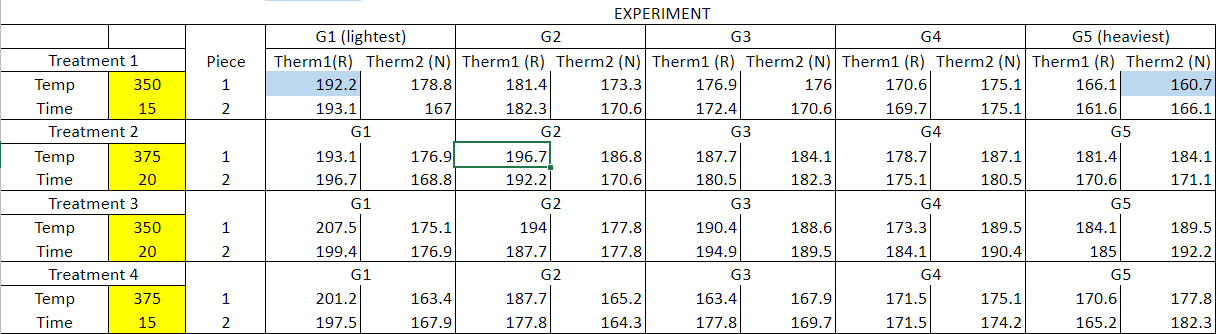
\includegraphics[scale=0.50]{Technical/data.png}
    \caption{Pre-processed data of internal temperature measurements, grouped by specific treatment (left). G1-G5 represent chicken pieces from corresponding weight groups 1-5. Two measurements of temperature were obtained from a single chicken piece by (R) and (N).}
\end{figure}

\par\hspace{0.5cm}For simplicity of the analysis, the average of each recorded internal temperature as the final internal temperature, for each experimental unit.
\par\hspace{0.5cm}To ensure a well-designed experiment, 4 principles of the experiment were considered: 
\begin{itemize}
        \item{\textbf{Control: }Experimental units were obtained from chicken breasts sourced from the same manufacturer (brand), prepared on the same day. Weight (mass) of chicken was considered by using the same number of pieces of similar weights (i.e. 2 from each of 5 weight groups) in each treatment. During the experiment, fluctuations in oven temperature were considered and controlled for by keeping the oven open and starting at room temperature before each treatment, then preheated for an identical period (2.5 minutes) each time. The baking tray was cooled down and cleaned at each treatment iteration, with fresh baking paper placed on top of it. Chicken pieces were arranged in an identical manner on the tray for each treatment, with 5 rows and 2 columns, corresponding to 5 weight groups (ordered from lightest to heaviest) of 2 pieces each. The pieces were placed in marked positions, a minimum of 4cm apart to maintain air flow around each piece. The tray was placed in the middle of the oven each time to ensure similar heat dispersion during cooking. Kitchen room temperature was monitored to remain at 24.5${^\circ}$C throughout the experiment.}
    \item{\textbf{Blocking: }No blocking was used in the experiment. The brand of chicken breasts and method of their preparation in the factory (halal) was controlled, however there was no supplementary information available to block the experimental units. Possible considerations could have been chicken age, diet, species or living conditions, which could have had an impact on internal meat fibre structure and temperature resistivity and permeability.
    \item{\textbf{Randomization: } Order of treatments was determined randomly. The 4 options were written on four pieces of paper and folded, then randomly chosen to form an order 1-4 by a blind-folded team member. For each weight group of cut chicken breast, there were 8 pieces. To choose 2 pieces for each of 4 treatments when preparing the baking tray, they were picked by a blind-folded team member from each weight group.}
    \item{\textbf{Replication: }Each treatment used  2 pieces from each cut-breast weight group, for 5 weight groups, thus the experiment was replicated ten times per treatment.}
\end{itemize}

%-----------------------------------------Analysis-------------------------------------
\section{Analysis} \label{Analysis}
\vspace{-0.25cm}
%-----------------------------------------Sample Size------------------------------------
\subsection{Sample Size}\label{Sample Size}
\vspace{-0.25cm}
\par\hspace{0.5cm} Assuming factors with a large effect of $f = 0.5$, a significance level of $\alpha = 0.10$, and a power of $1 - \beta = 0.8$, the R package "WebPower"\footnote{Specific code is listed in Appendix line 11 - 17} calculates the minimum total sample size to be $n = 33.3887$. The sample size in this study is 40, well above the minimum, it is deemed that the sample size is justified.
\vspace{-0.25cm}
%-----------------------------------------Assumptions------------------------------------
\subsection{Assumptions for linear model}\label{Assumptions for linear model}
\vspace{-0.25cm}
%-----------------------------------------Independence------------------------------------
\subsubsection{Independence}\label{Independence}
\vspace{-0.25cm}
\par\hspace{0.5cm}All experimental units are randomly assigned to each treatment, the order of all treatments are randomly assigned for the experiment, and all treatments are randomly assigned in order for the experiment. The methods of randomization were optimized, however their necessity could even be arguable since one experimental unit measurement does not have any effect on another subject's response value. 
\vspace{-0.25cm}
%-----------------------------------------Normality------------------------------------
\subsubsection{Normality Assumption}\label{Normality Assumption}
\vspace{-0.25cm}
\par\hspace{0.5cm}By the QQ plot and Shapiro-Wilk test of normality\footnote{Specific code is listed in Appendix line 58 - 62 and line 66-70}, it appears that, for the Additive Model, normality seems satisfied. For the Interaction Model, however, the QQ plot satisfies normality only some of the time. Closer examination of the interaction model is required during further analysis. 
\begin{figure}[h]
    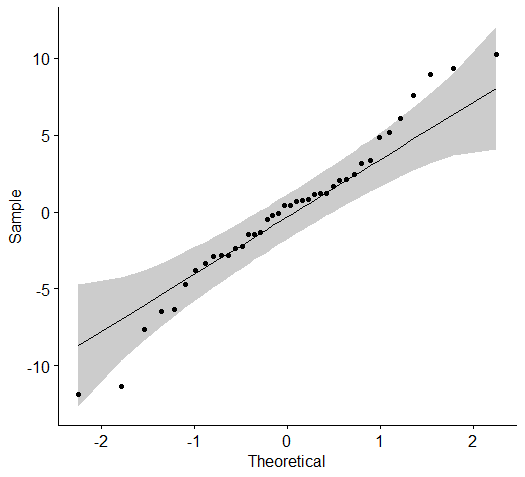
\includegraphics[scale=0.55]{Technical/Additive_qq.png}
    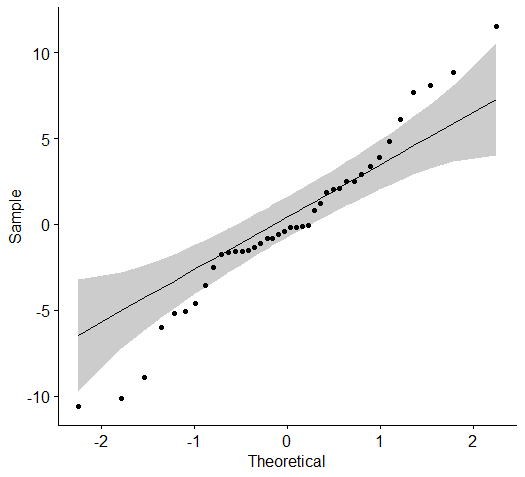
\includegraphics[scale=0.55]{Technical/Interaction_qq.png}
    \label{Additive Linear Model}
    \caption{Additive Model(Left), Interaction Model(Right)}
\end{figure}
$$H_0: \textbf{Data originates from normal distribution,  vs.} H_a: \textbf{Data does not originate from normal distribution}$$
\par\hspace{0.5cm}The Shapiro-Wilk test results in $p$-values of $0.495 > \alpha = 0.10$  and $ 0.427 > \alpha = 0.10$ for the Additive Model and Interaction Model respectively. Hence, with a significance level of 0.10, we fail to reject the null hypothesis. Therefore, it is concluded that the data originates from the normal distribution, satisfying the normality assumption.
%-----------------------------------------Variance------------------------------------
\subsubsection{Equal Variance}\label{Equal Variance}
\vspace{-0.25cm}
\par\hspace{0.5cm}Conduct Bartlett's Test\footnote{Specific code is listed in Appendix line 74} to check the Equal Variance assumption.
$$H_0: \sigma_{1}^2 = \sigma_{2}^2 = \sigma_{3}^2 = \sigma_{4}^2 \hspace{3pt} vs. \hspace{3pt} H_a: \sigma_{i}^2 \neq \sigma_{j}^2, j \neq k$$
Obtained a p-value of $0.1955 > \alpha = 0.10$ for Barlett's Test. Therefore we fail to reject the null hypothesis, all the groups within the data have the same variance. A boxplot could also be checked for visual confirmation of data distribution and variances: 
\vspace{-0.25cm}
\begin{figure}[h]
    \centerline{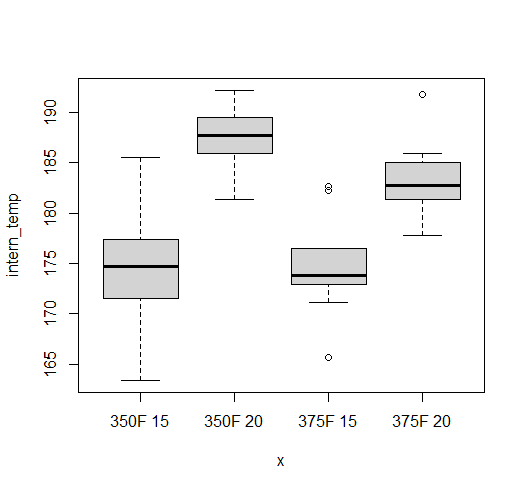
\includegraphics[scale=0.6]{Technical/boxplot.png}}
    \label{BoxPlot}
    \caption{BoxPlot of response data spread (y), per treatment (x).}
\end{figure}

\vspace{-0.25cm}
%-----------------------------------------Linear Models------------------------------------
\subsection{Linear Models}\label{Linear Models}
\vspace{-0.25cm}
\par\hspace{0.5cm}The experiment deals with two factors, both with two levels. Therefore, the best method use to conduct the analysis of factor signficance is Two-Way ANOVA. It was first investigated whether there exist any interaction between the factors of cooking time and cooking temperature. 
\begin{figure}[h]
    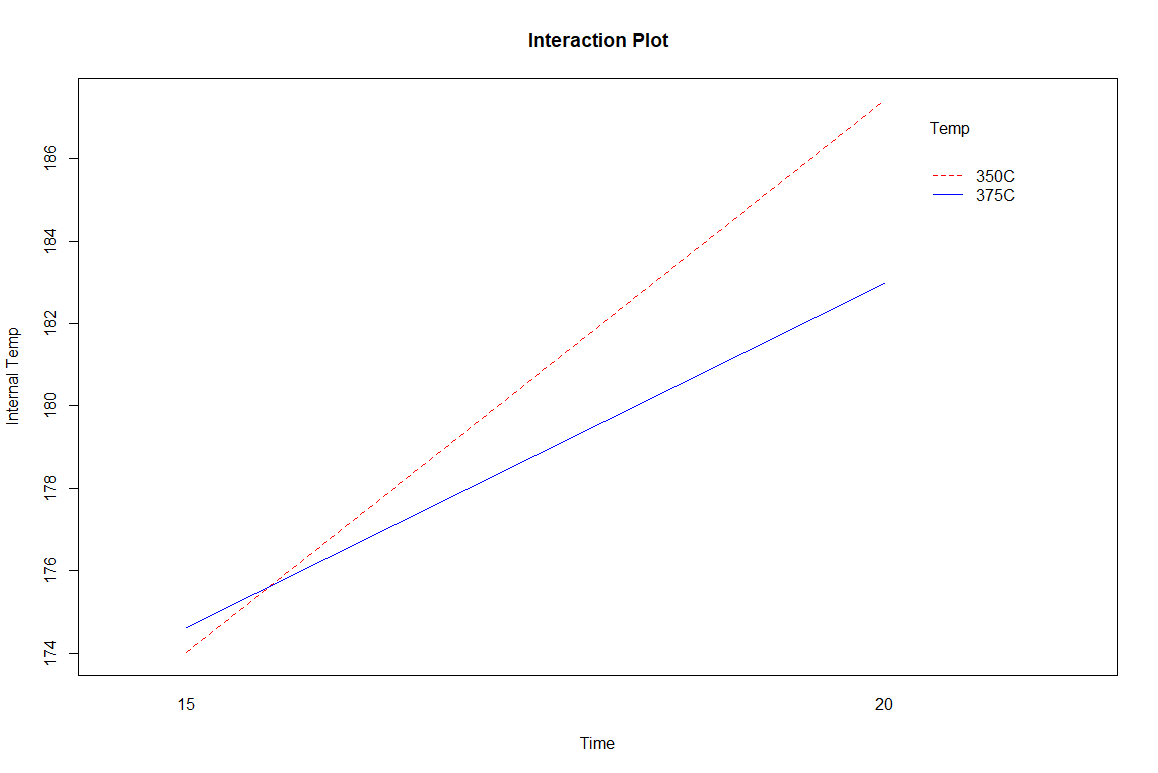
\includegraphics[scale=0.50]{Technical/interaction_plot.png}
    \label{figl}
    \caption{Interaction Plot}
\end{figure}
\par\hspace{0.5cm}By plotting the group mean, there exists a potential interaction by observation. A hypothesis is built to determine the interaction effect: $$H_0: (\alpha\beta)_{jk} = 0 \mbox{ for all j,k vs. } H_a: \mbox{at least one}(\alpha\beta)_{jk} ≠ 0.$$
\hspace{1cm}The data is then analyzed via Two-Way ANOVA. The p-value representing interaction effect is $0.1183 > \alpha = 0.10$. Therefore, fail to reject $H_0$ with the conclusion that the interaction effect between the factors is not significant.
Justifying that there exists no interaction effect, the additive model is used to test the main effects of factors:
$$\mbox{Oven Temperature Effect: } H_0: \alpha_j = 0 \mbox{ for all j vs. } H_a: \mbox{at least one} \alpha_j ≠ 0.$$
\par\hspace{0.5cm}The additive model shows that the p-value for temperature is $0.1183 > \alpha = 0.10$. As a result, fail to reject $H_0$ with the conclusion that the specific temperatures had no significantly different effect on the final internal temperature of chicken.
$$\mbox{Cooking Time Effect: } H_0: \beta_k = 0 \mbox{ for all k vs. } H_a: \mbox{at least one} \beta_k ≠ 0.$$
\par\hspace{0.5cm}The next line of the additive model gives us the p-value for Cooking Time, which is $6.227*10^{-08} < \alpha = 0.10$. It is highly unlikely to meet type I error, therefore it is concluded that the employed Cooking Times were a significant factor in final internal temperature of the chicken.


%-----------------------------------------Conclusion-----------------------------------
% \textcolor{red}{(I don't think we varied the temperature enough - Lucas)}
\section{Conclusion} \label{Conclusion}
\hspace{1cm}The main goals of this experiment were to determine whether oven temperature and cooking time were significant factors in predicting the internal temperature of pieces of cut chicken breast after cooking, and whether the effect of the oven temperature on the chicken breast's internal temperature depends on the different levels of oven cooking time and vice versa. From the analysis, it was concluded that the used cooking times were a significant predictor of the internal temperature of the pieces of chicken in comparison to the employed cooking temperatures. Furthermore, it was concluded that the effect of oven temperature on the chicken breast’s internal temperature does not depend on the different levels of oven cooking time and vice versa. Based on the results from this experiment, it is recommended to cook pieces of chicken breast in a 350 $^\circ$F oven for 15 minutes to achieve the best results. This combination of oven temperature and cooking time will lead to chicken cooked to a safe internal temperature while taking the least amount of time and being the least overcooked.
\newpage
%-----------------------------------------Appendix-----------------------------------
\section{Appendix} \label{Appendix}
\begin{lstlisting}[language=R]
# Install the necessary packages that will be used
# install.packages("ggplot2");
# install.packages("WebPower");
# install.packages("ggpubr");
# install.packages("rstatix");
library(rstatix)
library(WebPower);
library(ggpubr);

# Looking for a total sample size with an effect size of 0.5, a significant level of 0.10, and a power of 0.8
wp.kanova(ndf=2, f=0.4, alph=0.10, ng=4, power = 0.8);
Multiple way ANOVA analysis

           n ndf      ddf   f ng alpha power
    33.38887   2 29.38887 0.5  4   0.1   0.8
    
wp.kanova(n = 40, ndf=2, f=0.4, alph=0.10, ng=4);
Multiple way ANOVA analysis

     n ndf ddf   f ng alpha     power
    40   2  36 0.5  4   0.1 0.8676117
    
# Response variable - the internal temperature of the experimental unit 
y <- c(185.5, 180.1, 177.4, 176.5, 176.5, 
       171.5, 172.9, 172.4, 163.4, 163.9, 
       191.3, 188.2, 185.9, 182.8, 189.5, 
       192.2, 181.4, 187.3, 186.8, 188.6, 
       182.3, 182.7, 176.5, 171.1, 165.7, 
       173.8, 173.3, 172.9, 174.2, 173.8,
       185.0, 182.8, 191.8, 181.4, 185.9, 
       181.4, 182.9, 177.8, 182.8, 177.9)
# Two factors, Oven Temperature, and Oven Cooking Time
a <- factor(rep(c("350F", "375F"), each=20));
b <- factor(rep(c("15", "20"), each=10));
# construct the data frame
chicken <- data.frame(intern_temp=y, Temp=a, Time=b);
chicken <- within(chicken,{x <- paste(Temp, Time)});
# Group means of Oven Temperature 
with(chicken, tapply(intern_temp, Temp, mean));
  350F   375F 
180.705 178.800
# Group means of Cooking Temperature
with(chicken, tapply(intern_temp, Time, mean));
     15      20 
174.320 185.185 
# Cell Means
with(chicken, tapply(intern_temp, list(Temp, Time), mean));
          15     20
350F 174.01 187.40
375F 174.63 182.97
# Grand Means
mean_grand=mean(y);
mean_grand;
[1] 179.7525

# Additive model normality
additive_model<-aov(intern_temp~Temp+Time, data=chicken);
ggqqplot(residuals(additive_model));
shapiro_test(residuals(additive_model))
  variable                  statistic p.value
  <chr>                         <dbl>   <dbl>
1 residuals(additive_model)     0.975   0.495

# Interaction model normality
interaction_model<-aov(intern_temp~Temp*Time, data=chicken);
ggqqplot(residuals(interaction_model));
shapiro_test(residuals(interaction_model))
  variable                     statistic p.value
  <chr>                            <dbl>   <dbl>
1 residuals(interaction_model)     0.972   0.427

# Equal Variance Test for Both factors 
bartlett.test(intern_temp~x, data=chicken);
Bartlett test of homogeneity of variances
data:  intern_temp by x
Bartlett K-squared = 4.6955, df = 3, p-value = 0.1955

#BoxPlot
boxplot(intern_temp ~ x, data=chicken);

#Interaction Plot
with(chicken, interaction.plot(Time, Temp, intern_temp,
                            col=c("red", "blue"), main="Interaction Plot",
                            xlab="Time", ylab="Internal Temp"))

# Additive Model: Two-Way ANOVA
anova(lm(intern_temp ~ Temp + Time, data=chicken))
Analysis of Variance Table

Response: intern_temp
          Df  Sum Sq Mean Sq F value    Pr(>F)    
Temp       1   36.29   36.29  1.3983    0.2446    
Time       1 1180.48 1180.48 45.4851 6.227e-08 ***
Residuals 37  960.27   25.95
# Model with Interaction: Two-Way ANOVA
anova(lm(intern_temp ~ Temp*Time, data=chicken))
Analysis of Variance Table

Response: intern_temp
          Df  Sum Sq Mean Sq F value    Pr(>F)    
Temp       1   36.29   36.29  1.4573    0.2352    
Time       1 1180.48 1180.48 47.4031 4.649e-08 ***
Temp:Time  1   63.76   63.76  2.5602    0.1183    
Residuals 36  896.51   24.90             
\end{lstlisting}

\end{document}
